\begin{frame}
	\frametitle{Slides and Examples}

        \begin{itemize}
		\item Slides:\\
                  \url{https://depot.tu-dortmund.de/dlep3}
		\item Examples:\\ 
                  \url{https://depot.tu-dortmund.de/5al36} 
        \end{itemize}

\end{frame}

\begin{frame}
  \frametitle{About CMake}

        \begin{itemize}
          \item Open-source application for 'managing the build process' of a software package
          \item CMake is available on all major platforms (Linux, Windows, MacOS, ...) 
          \item Supports source directory trees that depend on multiple libraries
          \item CMake is a script language that includes almost all basic programming language elements
          \item CMake generates a native build environment for the OS it is executed on
          \item Supports in-place and out-of-place builds
          \item Can generate project files for various IDEs (Visual Studio, Xcode, Eclipse, ...)
          \item Has a mechanism to locate libraries in the OS
          \item 'Easy' to enable/disable optional components of a software package ($\rightarrow$ modular builds)
        \end{itemize}
\end{frame}

\begin{frame}
  \frametitle{Features of CMake}

        \begin{itemize}
          \item Saves a lot of time when building for different OSs 
          \item Easier to combine source code written in different languages 
          \item Easier to specify different build options 
          \item Widely used in many open-source packages
          \item Makes it easier to integrate third-party libraries
          \item cmake-gui as a graphical tool to help beginners and explore build options 
          \item ccmake to explore build options on the console 
          \item CDash as a built-in testing system and dashboard 
          \item CTest as a packaging system for the different operating systems 
        \end{itemize}

\end{frame}

\begin{frame}
  \frametitle{Software Packages that use CMake}
  \vspace{-1cm}

  \begin{columns}

    \column{0.5 \textwidth} {

      \begin{block}{Part of the Kitware Family}
        Used for building:
        \begin{itemize}
          \item VTK 
          \item ParaView 
        \end{itemize}
      \end{block}
      \begin{center}
      
\includegraphics[width=0.4 \textwidth]{img/kw-logo.png}
    \end{center}
    }
    \column{0.5 \textwidth} {
      \begin{block}{Open Source Libraries}
        \begin{itemize}
          \item Bullet Physics Enginge 
          \item CGAL 
          \item LAPACK 
          \item MikTeX 
          \item OGRE  
          \item OpenSceneGraph  
          \item Qt  
          \item Many solver packages (Eigen, Super-LU, ...)
          \item FeatFloWer  
          \item Feat3  
          \item ...  
        \end{itemize}
      \end{block}
    }
\end{columns}
\end{frame}

%\begin{frame}
%  \frametitle{Software Packages that use CMake}
%  \begin{tikzpicture}[remember picture,overlay]
%    \tikzset{shift={(current page.center)}}
%
%    \node[text width=8cm] (C1) at (-6.8, 2.5) {
%      \begin{block}{Part of the Kitware Family}
%        Used for building:
%        \begin{itemize}
%          \item VTK 
%          \item ParaView 
%        \end{itemize}
%      \end{block}
%    };
%
%    \node[text width=8cm] (C2) at (5,-1.6) {
%      \begin{block}{Open Source Libraries}
%        \begin{itemize}
%          \item Bullet Physics Enginge 
%          \item CGAL 
%          \item LAPACK 
%          \item MikTeX 
%          \item OGRE  
%          \item OpenSceneGraph  
%          \item Qt  
%          \item Many solver packages (Eigen, Super-LU, ...)
%          \item FeatFloWer  
%          \item Feat3  
%          \item ...  
%        \end{itemize}
%      \end{block}
%    };
%
%%    \node[text width=8cm] (C3) at (0,8) {
%%      \begin{block}{CMake}
%%        \begin{itemize}
%%          \item Script language to control the building process
%%          \item Generates a wide range of specific build files
%%        \end{itemize}
%%      \end{block}
%%    };
%%
%%    \node[text width=8cm] (C4) at (0,7) {
%%      \begin{block}{ParaView}
%%        \begin{itemize}
%%          \item VTK visualization by GUI
%%          \item Scripting via Python
%%          \item Extension by plugins
%%        \end{itemize}
%%      \end{block}
%%    };
%
%\end{tikzpicture}
%\end{frame}


\begin{frame}[fragile]
  \frametitle{CMake Simple Example}
  \vspace{-0.5cm}

  \begin{block}{CMakeLists.txt}
\begin{verbatim}
  cmake_minimum_required (VERSION 2.8)

  project(HelloWorld)

  set(mySources main.cpp)

  add_executable(HelloWorld ${mySources})

\end{verbatim}
\end{block}

\begin{center}
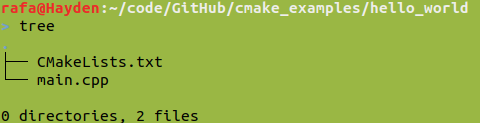
\includegraphics[width=0.8 \textwidth]{img/source-tree.png}
\end{center}

\end{frame}

\begin{frame}
  \frametitle{Out-Of-Source-Builds}
  \begin{itemize}
    \item Source files are in a different directory than the binary files 
  \end{itemize}

  \begin{center}
    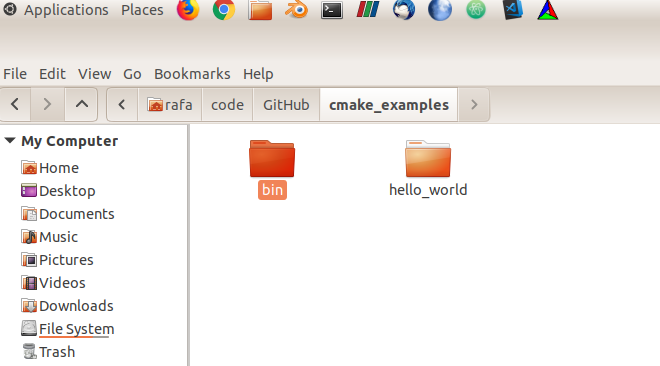
\includegraphics[width=0.8 \textwidth]{img/source-bin.png}
  \end{center}

\end{frame}

\begin{frame}
  \frametitle{Simple CMake Build Procedure}
  \begin{center}
    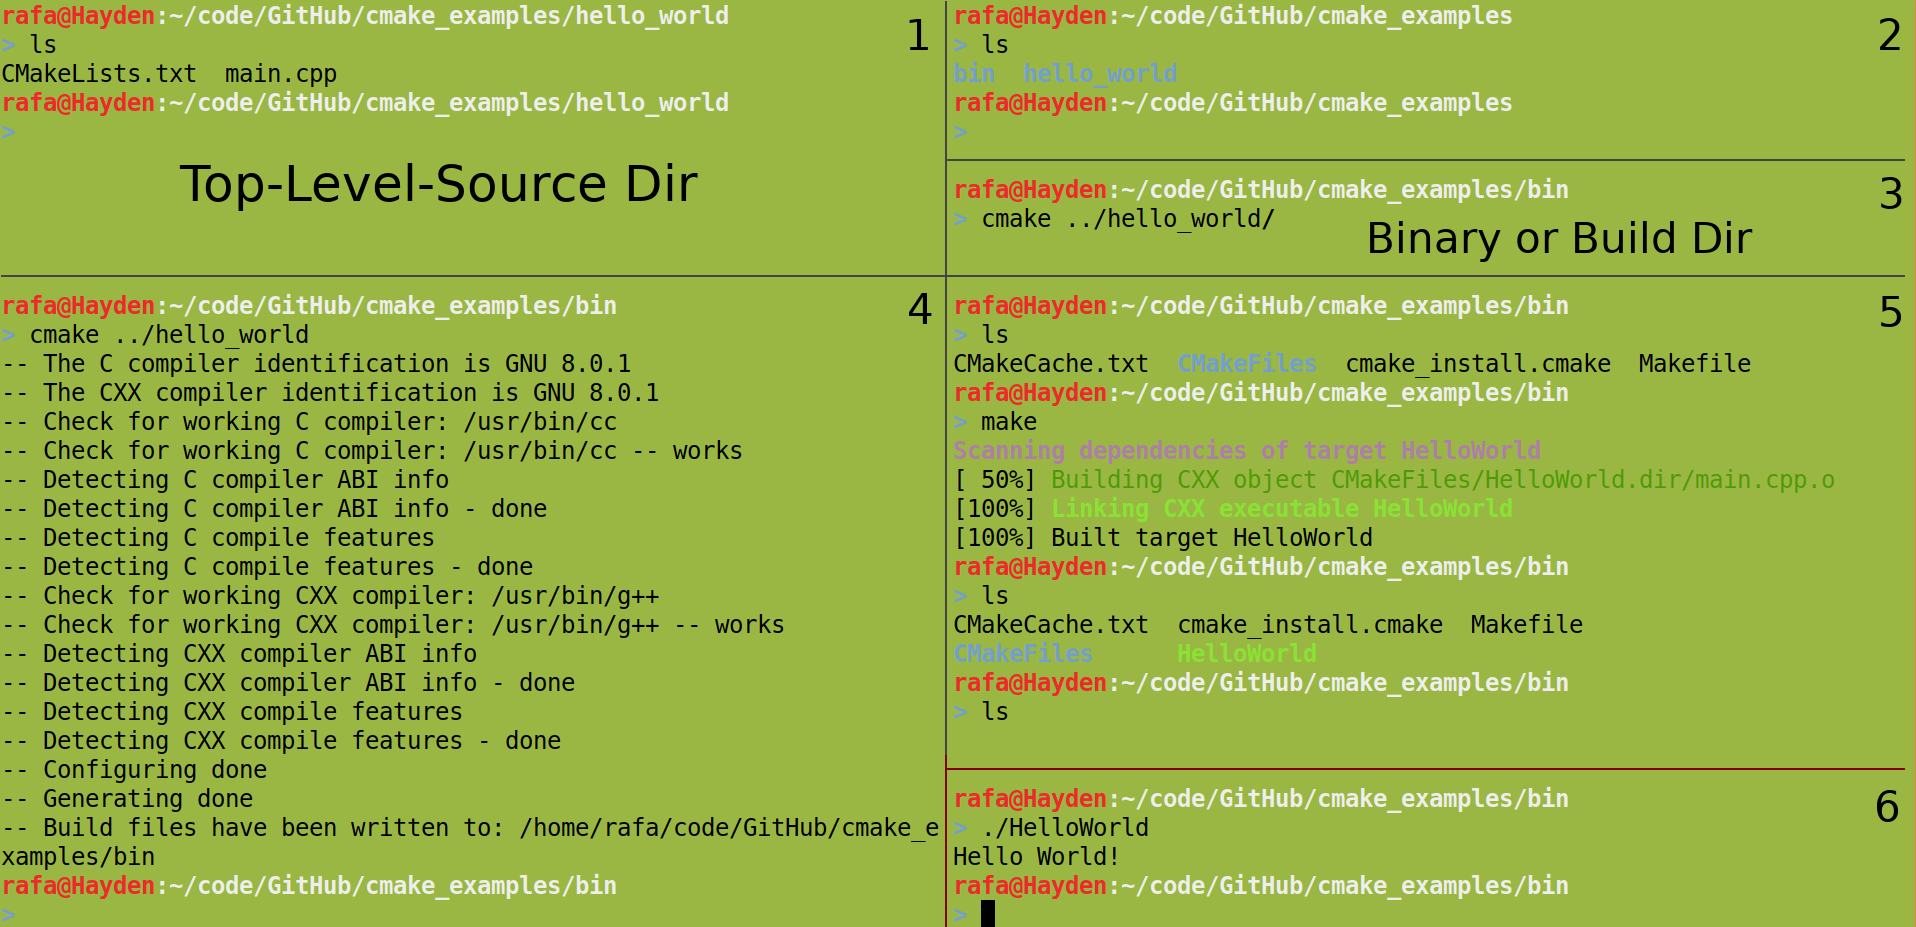
\includegraphics[width=\textwidth]{img/cmake-command-line.png}
  \end{center}
\end{frame}

\begin{frame}
  \frametitle{Simple CMake Build Procedure II}

    \begin{itemize}
      \item Searches for a file 'CMakeLists.txt' in the top level source directory as entry point 
      \item Two step process: 
      \begin{itemize}
        \item Configure step: parses the CMakeLists.txt files and stores information in CMake cache
        \item Generation of the OS specific build files based on the CMakeLists.txt
      \end{itemize}
      \item CMake Syntax: https://cmake.org/cmake/help/v3.13/manual/cmake-language.7.html
      \item For more complex source trees, subdirectories can be added with the \texttt{add\_subdirectory()} command
      \item Subdirectories added via \texttt{add\_subdirectory()} then need their own CMakeLists.txt file
      \item For each directory that contains a CMakeLists.txt a corresponding directory is created in the build directory tree
    \end{itemize}

\end{frame}

\begin{frame}[plain]
  \frametitle{CMake GUI}

  \begin{center}
    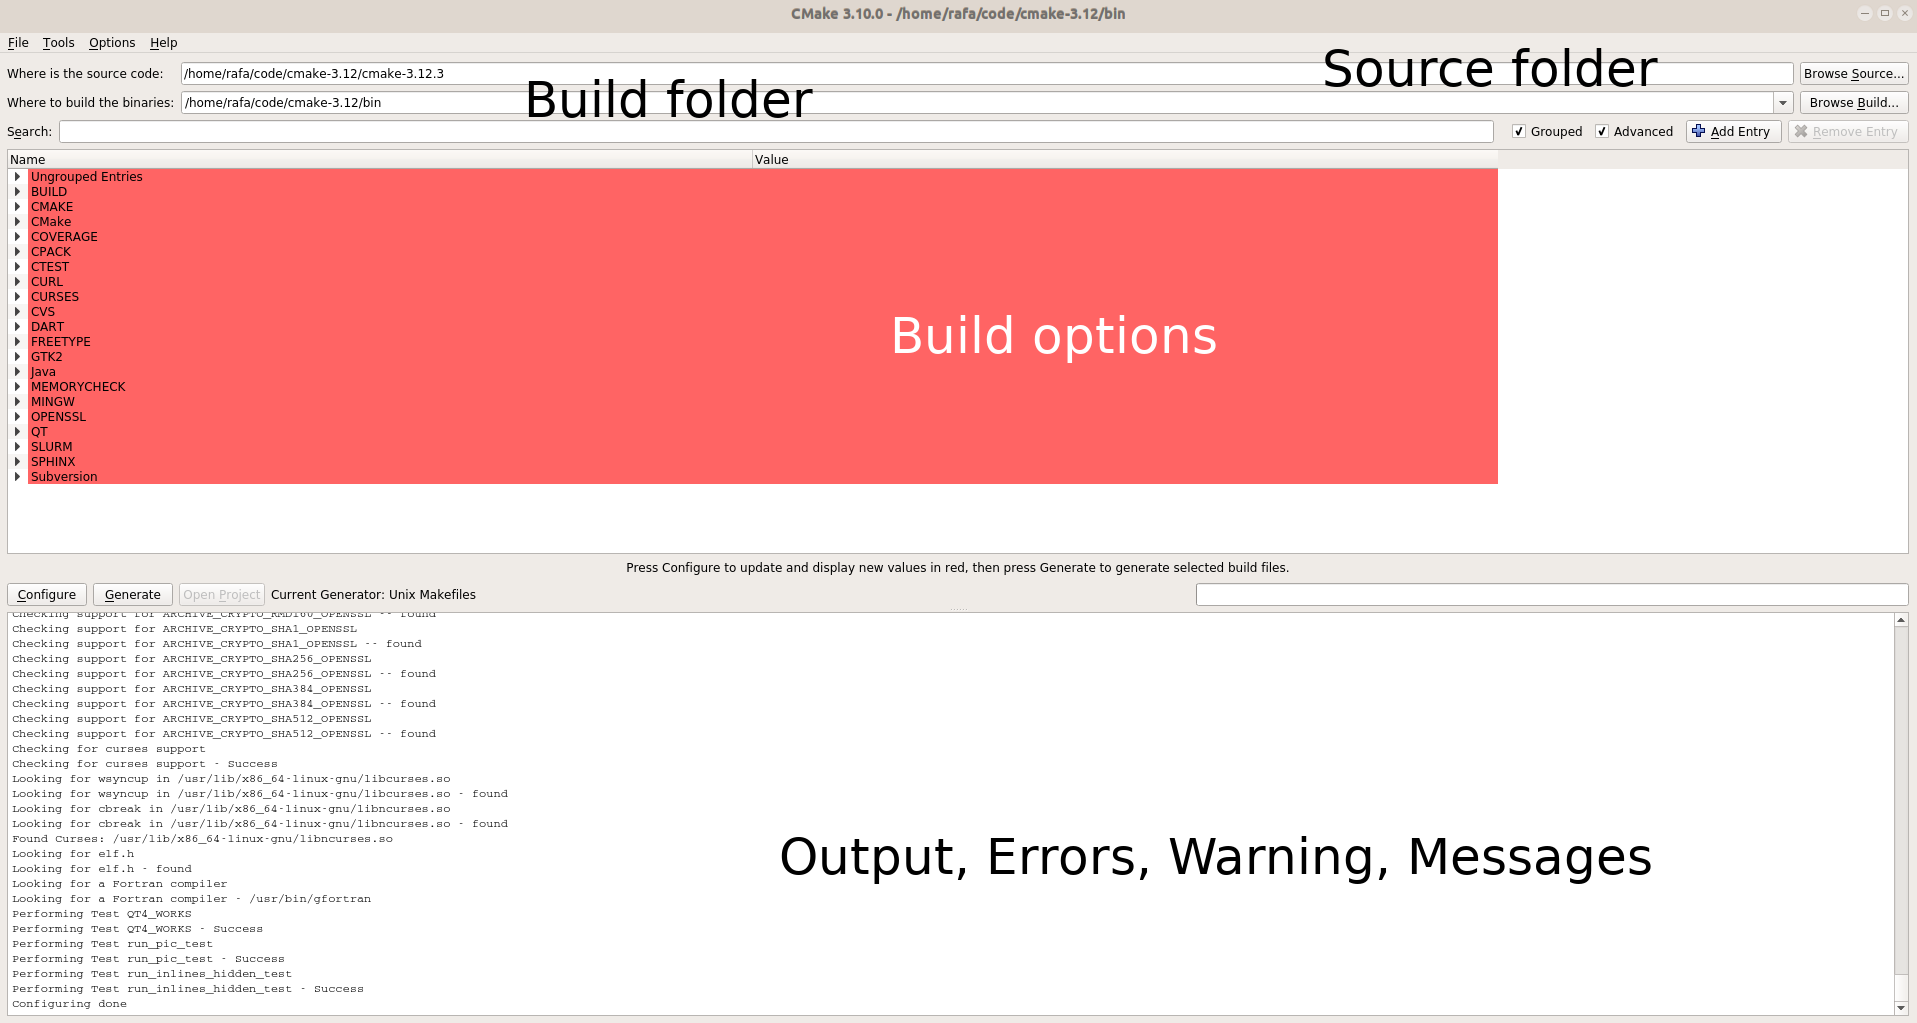
\includegraphics[width=\textwidth]{img/cmake-gui.png}
  \end{center}

\end{frame}

\begin{frame}[fragile]
  \frametitle{Advanced CMake Example}

    \begin{itemize}
      \item Multiple source folders
      \item Add a user defined library  
      \item Search for third-party libraries
    \end{itemize}

  \begin{columns}
    \column{0.5 \textwidth} {
      \begin{center}
        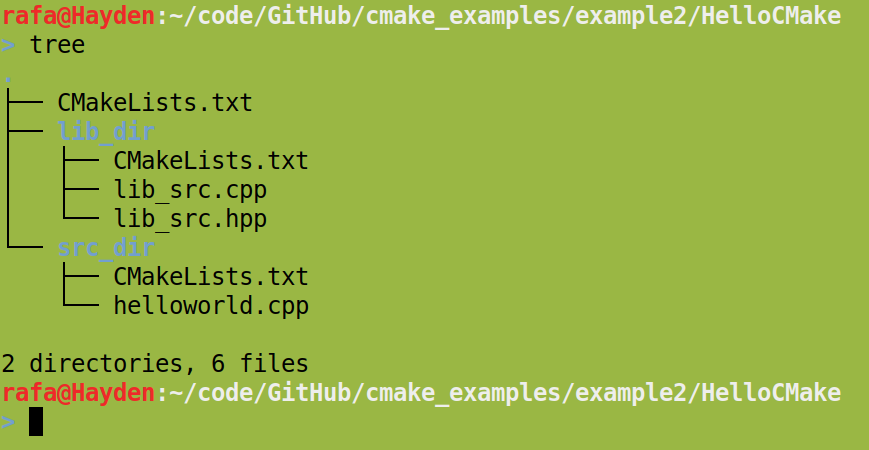
\includegraphics[width=1.0 \textwidth]{img/adv-cmake-dir.png}
      \end{center}
    }
    \column{0.5 \textwidth} {
      \begin{center}
        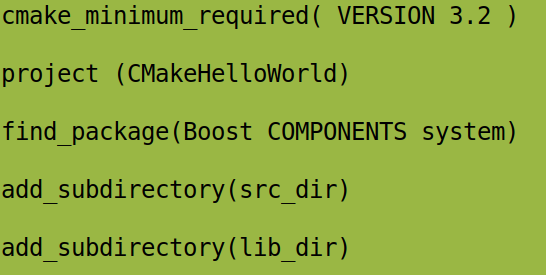
\includegraphics[width=1.0 \textwidth]{img/adv-cmake-code.png}
      \end{center}
    }
\end{columns}

\end{frame}

\begin{frame}[fragile]
  \frametitle{Building a custom library}
  \begin{block}{The lib\_dir CMakeLists.txt}
\begin{verbatim}
set (LIB_SOURCE lib_src.cpp lib_src.hpp)

add_library(hello_lib ${LIB_SOURCE}) 

target_compile_definitions(hello_lib PRIVATE FOO=1)

target_include_directories(hello_lib PUBLIC .)
\end{verbatim}
  \end{block}

\begin{itemize}
  \item Set the include paths or include directories
  \item Add defines that can be used by the preprocessor 
\end{itemize}
  
\end{frame}

\begin{frame}[fragile]
\begin{block}{The src\_dir CMakeLists.txt}
\begin{verbatim}
set (MAIN_SOURCE helloworld.cpp)
add_executable(hello_world ${MAIN_SOURCE})
target_compile_options(hello_world PRIVATE -Wall -Wextra)
if (Boost_FOUND)
  target_compile_definitions(hello_world PRIVATE BAR=1 
  WITH_BOOST=1)
  target_include_directories(hello_world PRIVATE 
  ${CMAKE_SOURCE_DIR}/lib_src ${BOOST_INCLUDE_DIRS})
else(Boost_FOUND)
  target_compile_definitions(hello_world PRIVATE BAR=1)
  target_include_directories(hello_world PRIVATE 
  ${CMAKE_SOURCE_DIR}/lib_src)
endif (Boost_FOUND)
target_link_libraries(hello_world hello_lib)
\end{verbatim}
\end{block}

\end{frame}

\begin{frame}
  \frametitle{CMake - Compilation Flags}
  \begin{block}{Settings Compiler Flags}
    \begin{itemize}
      \item Before CMake version 2.8.12 compilation flags were set by:
      \begin{itemize}
        \item Using the global variable \texttt{CMAKE\_<LANG>\_FLAGS\_<CONFIG>}, i.e. \texttt{CMAKE\_C\_FLAGS\_RELEASE}  
        \item The command \texttt{add\_compile\_options}
      \end{itemize}
    \item Not recommended anymore, \texttt{CMAKE\_<LANG>\_FLAGS\_<CONFIG>} is global
    \item Error prone and 'messy' if you have different targets that require different compilation flags
    \item Since CMake version 2.8.12 it is recommended to use \texttt{target\_compile\_options} sets flags for each individual target
    \item The optimization level is automatically set by CMake when setting the build type:
      \begin{itemize}
        \item \texttt{CMAKE\_BUILD\_TYPE}=Release $\Longrightarrow$ "-O3"
        \item \texttt{CMAKE\_BUILD\_TYPE}=Debug $\Longrightarrow$ "-g"
      \end{itemize}
    \end{itemize}
  \end{block}
\end{frame}

\begin{frame}
  \frametitle{CMake Find Modules}

    \begin{itemize}
      \item CMake has a set of \textbf{CMake modules} to find common third-party libraries
      \item User can provide additional \textbf{CMake modules} to locate libraries 
      \item A \textbf{CMake module} is a *.cmake file written in the CMake language 
      \item Naming convention for module files: \texttt{FindLIBRARY.cmake} 
      \item A custom module needs to be added to the module path 
      \item Module by convention set variables:
    \begin{itemize}
      \item myLibrary\_FOUND: was the library found or not 
      \item myLibrary\_INCLUDE\_DIRS: the include directories of the library  
      \item myLibrary\_LIBRARY\_DIRS: the directories where the libraries are located  
      \item myLibrary\_LIBRARIES: the path to libraries  
      \item ... (see CMake reference on modules)  
    \end{itemize}
    \end{itemize}

\end{frame}

\begin{frame}

  \frametitle{External Projects}


\end{frame}

\begin{frame}

  \frametitle{Configuration of Tracer Filters}

    \begin{itemize}
      \item Tracer type filters need an \keyword{input data set} and a \keyword{seed source}
      \item The input data set is the the flow field  
      \item The seed source is a user-defined starting location for the particles inside the flow field  
    \end{itemize}
    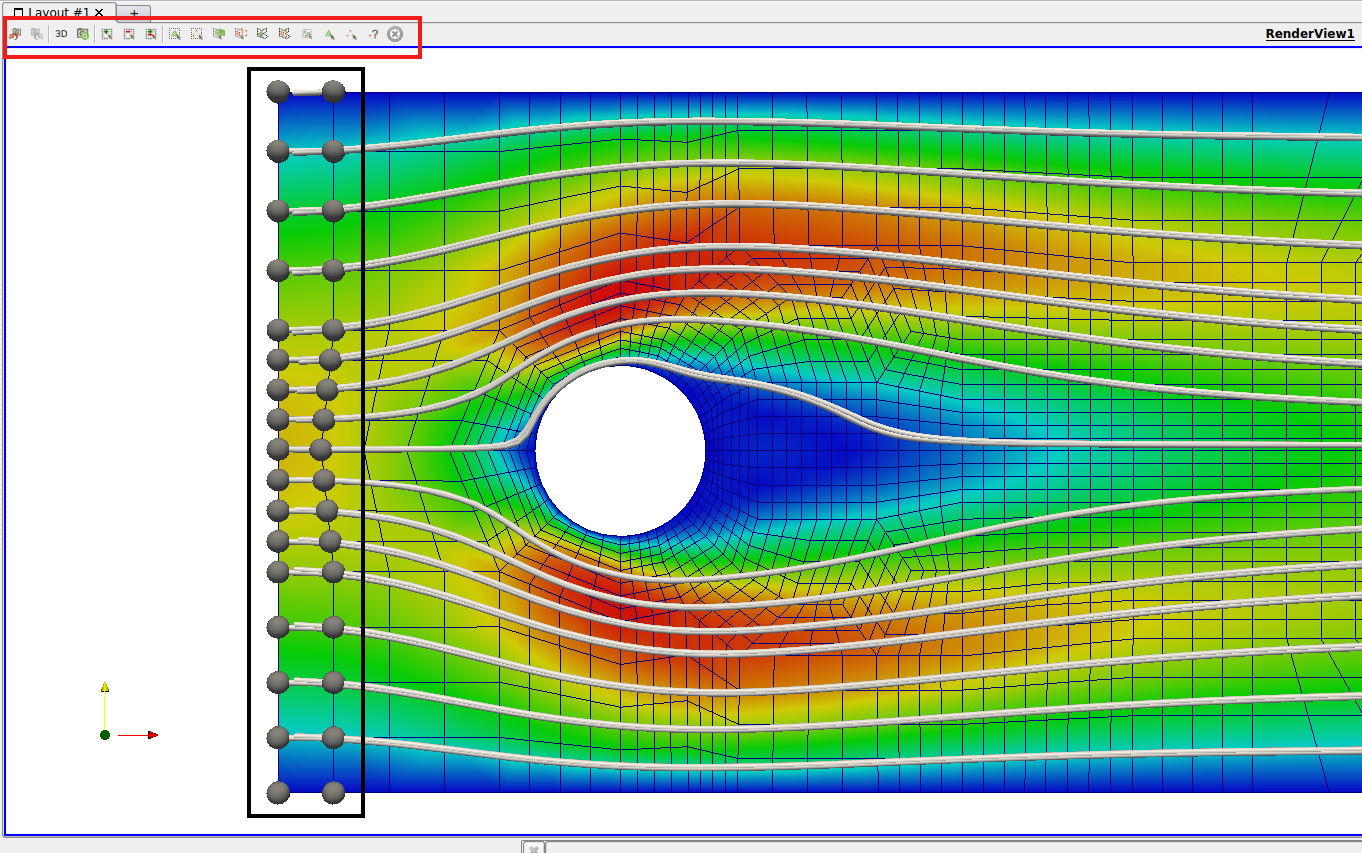
\includegraphics[width=0.5\textwidth]{screenshots/tracer-source.png}

\end{frame}

\begin{frame}

  \frametitle{Advanced Filters: Particle Tracer}

    \begin{itemize}
      \item Used to visualize transient flow data by particles 
      \item A particle path is produced by moving a particle along successive vector fields 
      \item Particle movement can then be animated by the \keyword{Animation Control} 
      \item Particle tracer example location: \kommandozeile{/mypath/to/examples/pv\_examples/AdvancedFilters/particle\_tracer}
    \end{itemize}
    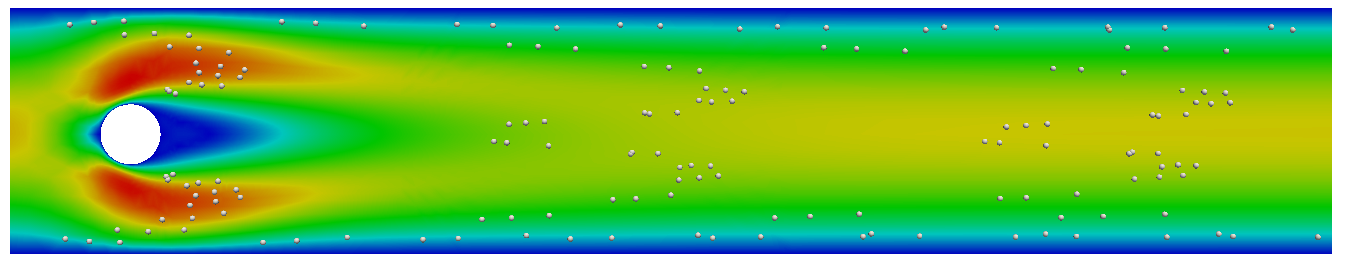
\includegraphics[width=\textwidth]{screenshots/particle-tracer.png}

\end{frame}

\begin{frame}

  \frametitle{List of Useful Filters}

    \begin{itemize}
      \item \keyword{Extract Selection}: Extract a subset from a data set (tracer source, plotting, etc)
      \item \keyword{Extract Surface}: Generates a polygonal surface mesh (exporting, rendering, remeshing) 
      \item \keyword{Clean to Grid}: Removes multiply defined simplices and converts to unstructured mesh
      \item \keyword{Integrate Variables}: Performs numerical integration of the fields defined in the data set on the mesh 
      \item \keyword{Iso-Volume or Iso-Surface}: Constructs a volume or a surface from a function defined on the mesh 
      \item \keyword{Plot Over Line}: Generates a plot of data fields along a line (inflow profiles, etc.) 
      \item \keyword{Calculator}: Use a set of mathematical operations to compute a new data field from existing ones (often used together with integrate variables filter)
    \end{itemize}

\end{frame}

\begin{frame}

  \frametitle{Input Data Formats}

    \begin{itemize}

      \item VTK data formats support polygonal data sets and structured or unstructured meshes 

      \item \keyword{VTK Legacy format .vtk} is a simple format useable for unstructured meshes (not suited for distributed data)  

      \item \keyword{VTK unstructured .vtu} is an xml based format for unstructured meshes   
    \begin{itemize}

      \item Can have the mesh data part encoded in a binary format   

      \item A \keyword{.pvtu} file can be used to reference the partial solutions of a distributed computation   

      \item A \keyword{.pvd} file can be used to add time information   

    \end{itemize}

    \item For further information on VTK file formats see:
      \url{http://www.vtk.org/VTK/img/file-formats.pdf}

  \end{itemize}

\end{frame}

\begin{frame}

  \frametitle{Scripted Postprocessing in ParaView}

  \begin{itemize}

    \item Python interface to access ParaView functionality by scripts

    \item Can be done interactively via a python shell: \keyword{Tools->Python Shell} 

    \item In a 'batch' style by passing a script to the executables \keyword{pvpython} or \keyword{pvbatch} 

    \item Documentation of the ParaView Python interface is under construction at:
      \url{https://www.paraview.org/ParaView3/Doc/Nightly/www/py-doc/}

    \item A trace mechanism is available to generate a PvPython script from a sequence of actions

    \item Beginners should use the trace mechanism (\keyword{Tools->Start Trace}) with the settings \keywords{Show Incremental Trace} and \keywords{only user-modified properties} 

    \item Upon \keyword{Tools->Stop Trace} a file is generated showing the PvPython script equivalent of the user's GUI actions
  \end{itemize}

\end{frame}

\begin{frame}

  \frametitle{PvPython Simple Example}

  \begin{itemize}
      \item PvPython simple example location: \kommandozeile{/mypath/to/examples/pv\_examples/PvPython/paraview\_python}

      \item Navigate to the folder and execute the PvPython script by: \kommandozeile{pvbatch ./python\_test.py \$(pwd)} or for versions higher than 5.1
        \kommandozeile{pvbatch {-}{-}use-offscreen-rendering ./python\_test.py \$(pwd)}

      \item The script will write an image \keyword{res.png} to the directory where you executed it 
      \item \keyword{Exercise:} Try to recreate the python script using the trace mechanism, compare the output images if they are the same.

      \item \keyword{Hint:} Prefer \keyword{pvbatch} over \keyword{pvpython} as pvpython tries to open an X windows which may fail on some computers    
  \end{itemize}

\end{frame}

\begin{frame}

  \frametitle{When to use PvPython}

  \begin{itemize}

    \item Repeated application of filters to a lot of different data sets (parameterize script w.r.t. data set) 

    \item Repeated application of operations that cannot be parametrized by ParaView GUI

    \item Perform an operation that cannot easily be done by ParaView filters 

    \item Quickly and repeatedly generate an ouput of a running simulation 

    \item Generate outputs on remote clusters 

    \item \keyword{ParaView Programmable Filter} or \keyword{Python Calculator} may serve as an alternative 

  \end{itemize}

\end{frame}

\begin{frame}

  \frametitle{Plotting with ParaView}

  \begin{itemize}

      \item PV plotting example: \kommandozeile{/mypath/to/examples/pv\_examples/Plotting/plotting.pvsm}

      \item Common ParaView plotting filters:
      \begin{itemize}

        \item \keyword{Plot Data} 

        \item \keyword{Plot Over Line} 

        \item \keyword{Plot Selection Over Time} 

      \end{itemize}

    \item Data can be exported to .csv to use in your favorite plot generator \keyword{File->Save Data}

    \item ParaView will by default export ALL data fields to the .csv file (even those that you do not want or need for the plot) 

    \item \keyword{Solution 1:} use <awk> to select the data columns you want: \kommandozeile{awk -F \textquotesingle,\textquotesingle $\;$  \textquotesingle\{print \$1 " " \$4\}\textquotesingle} (extract first and fourth column)

    \item \keyword{Solution 2:} Remove unneccessary fields before export: \kommandozeile{/mypath/to/examples/pv\_examples/Plotting/plotting2.pvsm}

  \end{itemize}

\end{frame}

\begin{frame}
  \frametitle{Client-Server Mode}

    \begin{itemize}
      \item In default mode ParaView is both the client and the server
      \item When client/server are different rendering and data processing can
        be handled by different computers 
      \item Simple X forwarding works adequately only if the network speed is fast
      \item Client-Server is preferable to access data on remote (non-local) clusters 
      \item Client-Server steps: \keyword{port forwarding}, \keyword{starting the remote server}, \keyword{connecting the client to the server}  
    \end{itemize}

    \begin{block}{Port Forwarding}
        \begin{itemize}
          \item Establish an ssh tunnel to forward the local port to the remote server: \\  
          \kommandozeile{> ssh lidong1.itmc.tu-dortmund.de \textbackslash}
          \kommandozeile{-L 11111:lidong1.itmc.tu-dortmund.de:11111}
        \end{itemize}
    \end{block}

\end{frame}

\begin{frame}
  %\frametitle{Client-Server Mode II}

    \begin{block}{Start the remote Server}
        \begin{itemize}
          \item Start a ParaView data server on the remote machine  
            \kommandozeile{> pvserver {-}{-}server-port=11111 {-}{-}use-offscreen-rendering}
        \end{itemize}
    \end{block}

    \begin{block}{Connect to the remote Server}
        \begin{itemize}
          \item Start a ParaView client locally  
          \item Press the <Connect> button on the toolbar  
          \item Manually configure the Server dialog:
          \begin{itemize}
            \item Name: myname   
            \item Server Type: Client/Server  
            \item Host: localhost 
            \item Port: 11111 
          \end{itemize}
        \end{itemize}
    \end{block}
  Pitfalls:
    \begin{itemize}
      \item You \textbf{have to} make use the same ParaView version of the client and the server
      \item Check that the port is not occupied, otherwise use a different port: 
      \kommandozeile{> lsof -i:11111}
    \end{itemize}

\end{frame}

\begin{frame}

  \frametitle{Additional ParaView Resources}

  \begin{itemize}
      \item ParaView documentation:\\
        \url{https://www.paraview.org/documentation/}
      \item ParaView Wiki:\\
        \url{https://www.paraview.org/Wiki/ParaView}
      \item ParaView Tutorial:\\
        \url{https://www.paraview.org/Wiki/The\_ParaView\_Tutorial}
      \item ParaView Mailing List:\\
        \url{https://public.kitware.com/mailman/listinfo/paraview}
      \item ParaView Catalyst:\\
        \url{https://www.paraview.org/Wiki/ParaView/Catalyst/Overview}
      \item ParaView Web JavaScript:\\
        \url{www.paraview.org/Wiki/ParaViewWeb\_JavaScript\_Introduction}
  \end{itemize}

\end{frame}

